\documentclass[a4paper,12pt]{report}
\usepackage{graphicx}
\title{Tugas Database 2}
\author{Idam fadilah}
\begin{document}

\maketitle
\chapter{Apex}
\section*{Oracle APEX}
\paragraph{}
Oracle APEX adalah platform pengembangan low-code yang memungkinkan anda membangun aplikasi perusahaan yang dapat diskalakan dan aman dengan fitur word-class yang dapat digunakan dimana saja.
\section*{Low code}
\paragraph{}
Low-code adalah cara cepat mendesain dan mengembangkan aplikasi software dengan sedikit coding manual. Dengan low-code, seorang pengembang aplikasi dapat memberikan nilai dengan lebih cepat dan lebih tepat. keuntungan low code :
\begin{itemize}
	\item mudah dijalankan
	\item sangat produktif
	\item scalable
	\item dapat diperpanjang
	\item kaya akan fungsionalitas dengan kode yang lebih sedikit
\end{itemize}
\section{sulitnya mengelola data dalam spreadsheet}
 kelemahan spreadsheet :
\begin{itemize}
	\item validasi data - manual dan rawan kesalahan
	\item integritas data - tidak dapat menjamin keakuratan dalam multi-user environment
	\item keamanan data - cell locking tidak efektif
	\item berbagi data - excel lamban dan sulit untuk dibagikan
\end{itemize}
\subsection*{Jenis aplikasi yang cocok untuk Oracle APEX}
jenis aplikasi :
\begin{itemize}
	\item Aplikasi dalam skala besar untuk ribuan pengguna
	\item Mengisi kekosongan dalam system perusahaan
	\item Merampingkan proses bisnis yang sudah ketinggalan zaman
	\item Modernisasi legacy system
	\item Aplikasi swalayan untuk semua karyawan
	\item Aplikasi responsif yang berfungsi pada perangkat apapun
	\item Bukti dari konsep
	\item Mengganti spreadsheet 
\end{itemize}
\section*{cara membuat workspace Oracle APEX}
\paragraph{}
\begin{itemize}
	\item Ketik link "https://apex.oracle.com/en/" dibrowser masing masing	
	\item klik "Get started for free"
	\item klik "Request a Free Workspace"\\	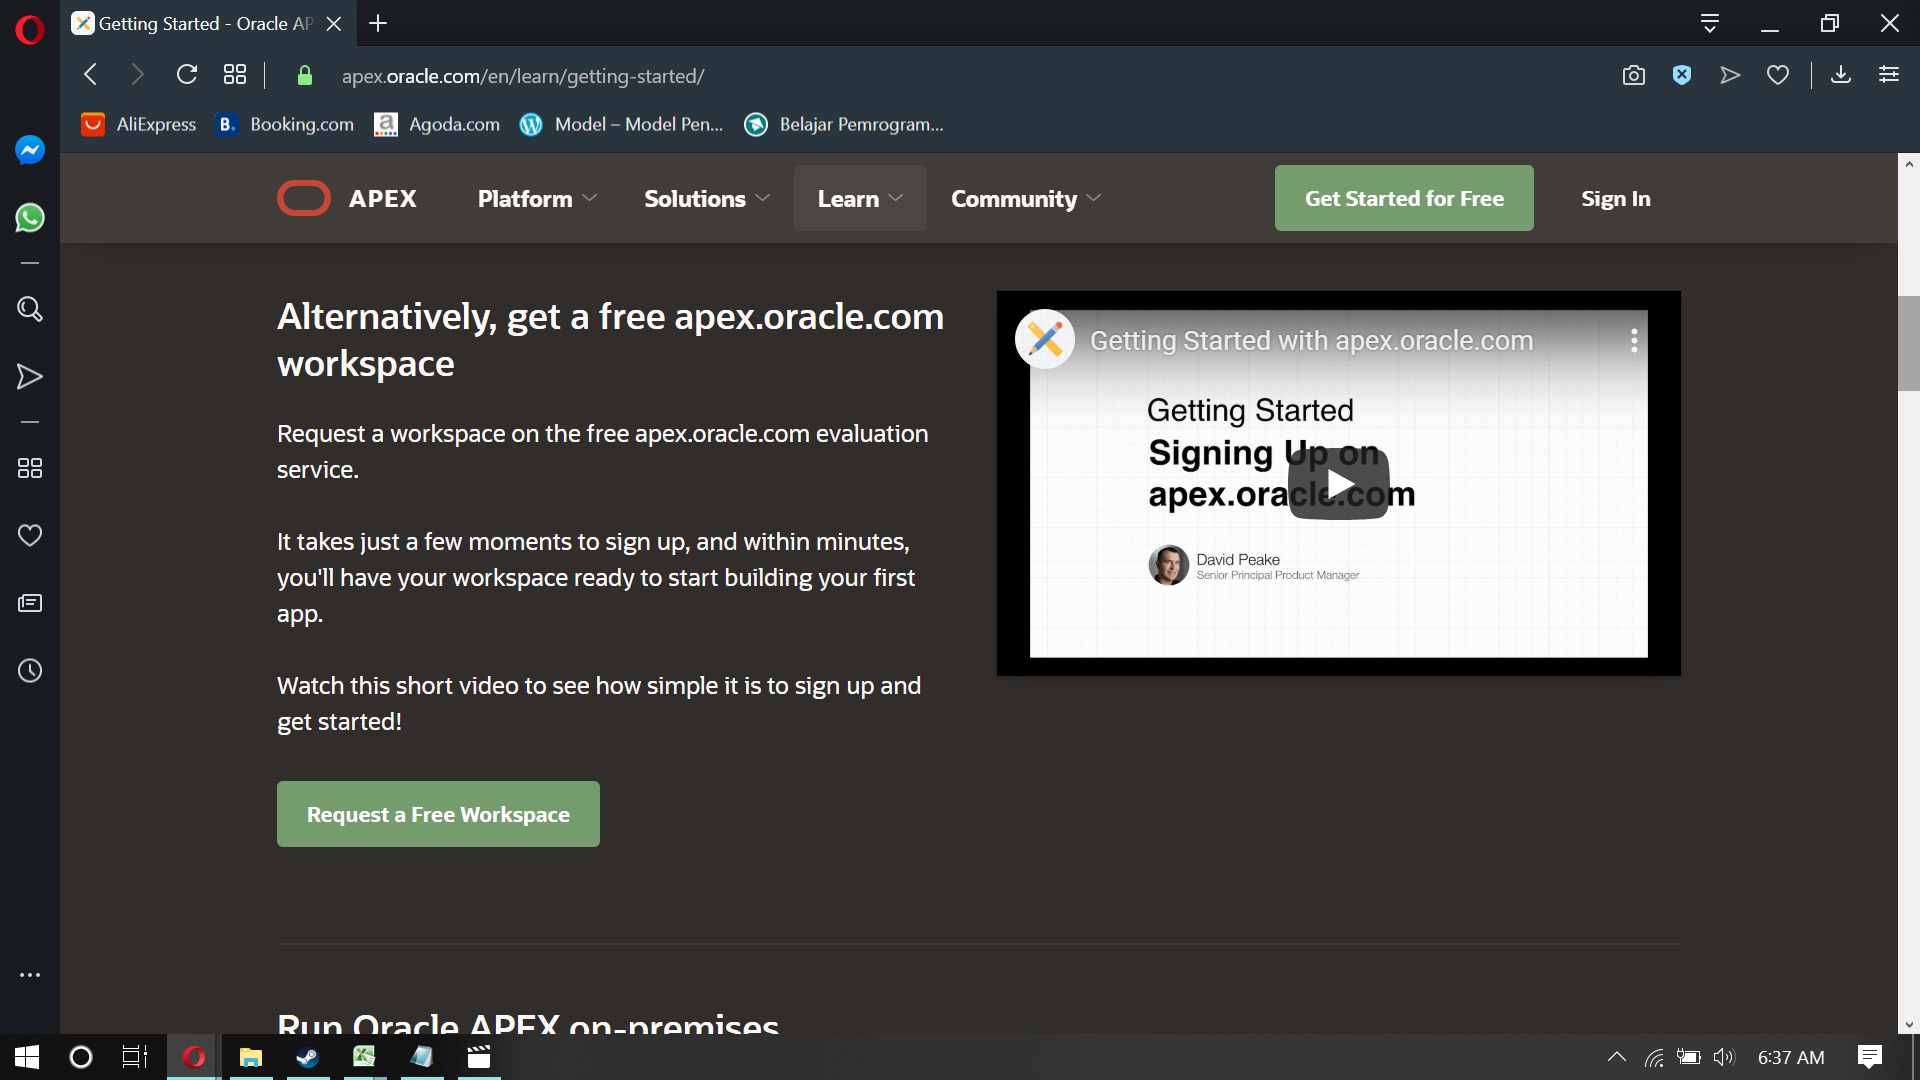
\includegraphics[width=12cm]{gambar/Screenshot (106).png} 
	\item Isi form sesuai dengan yang dibutuhkan, lalu klik next\\	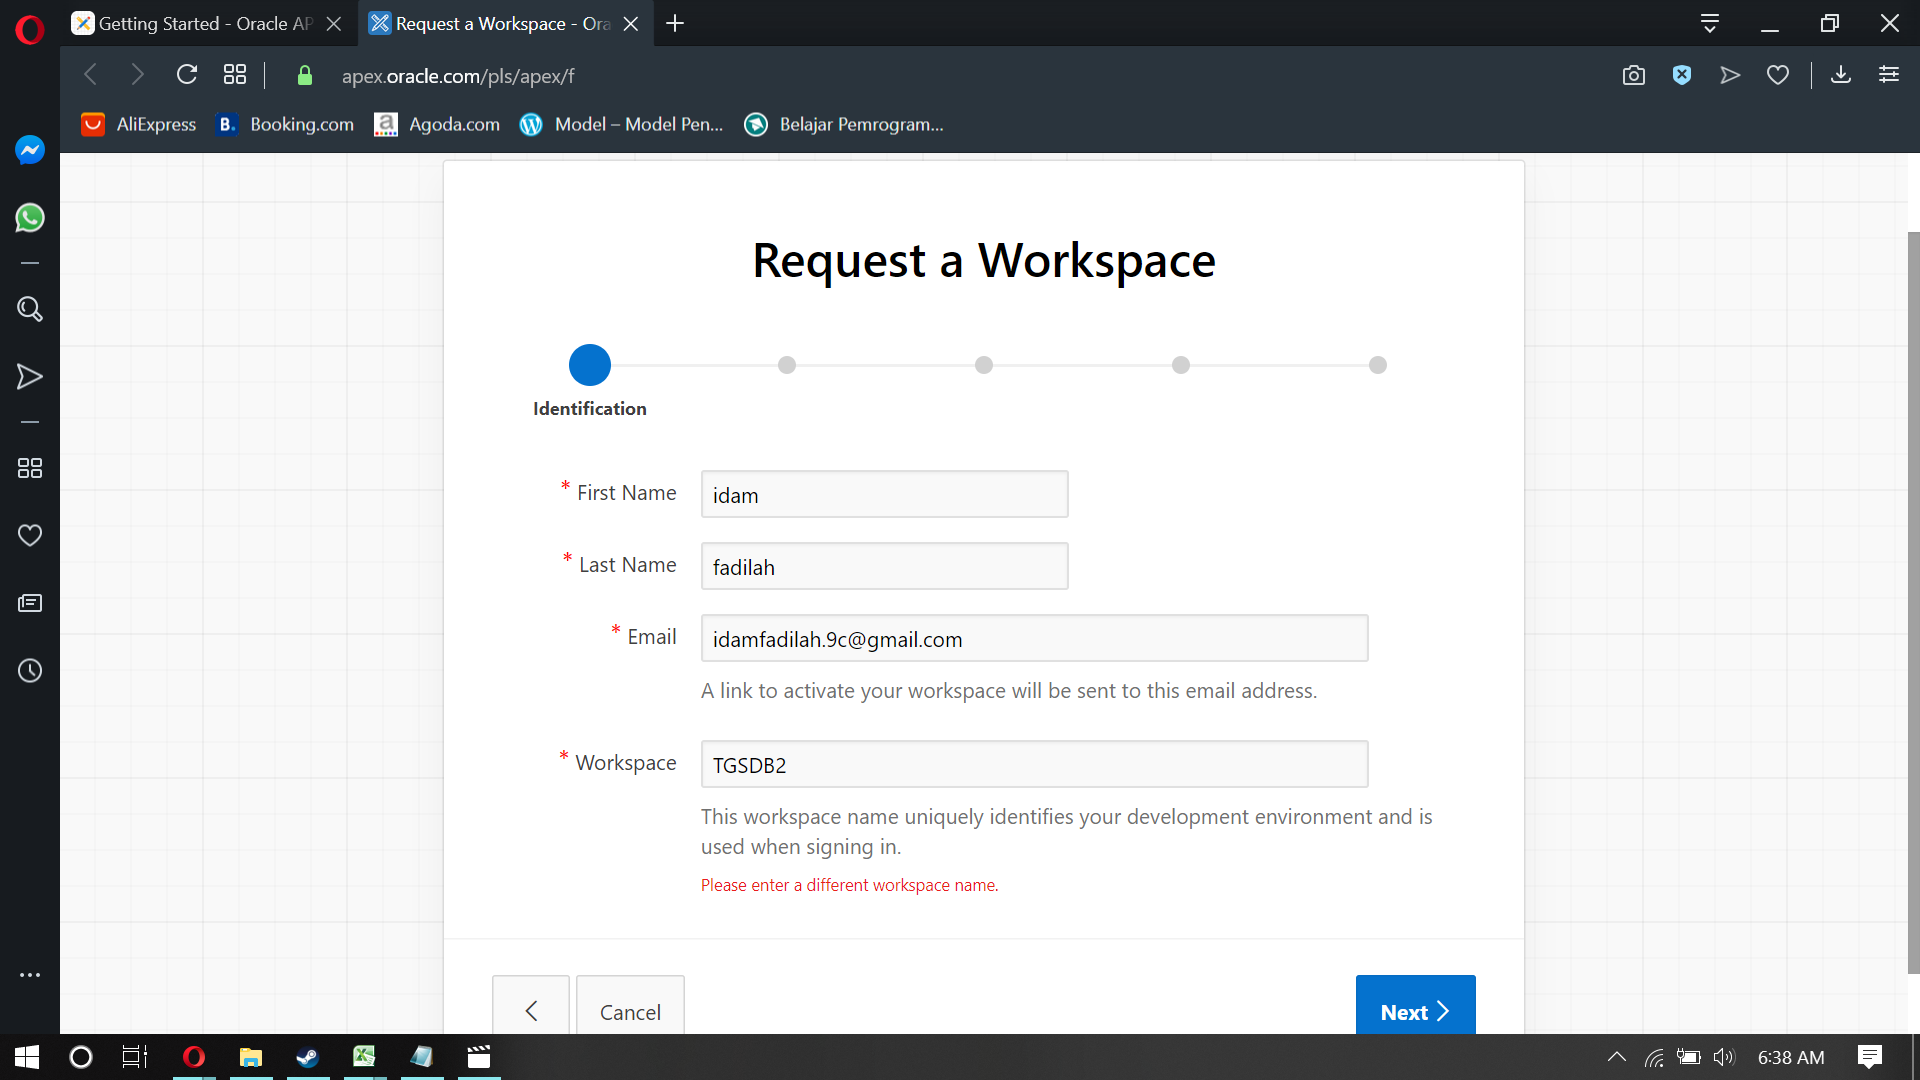
\includegraphics[width=12cm]{gambar/Screenshot (108).png} 
	\item Cetang "yes" pada kedua penyataan, lalu klik next\\	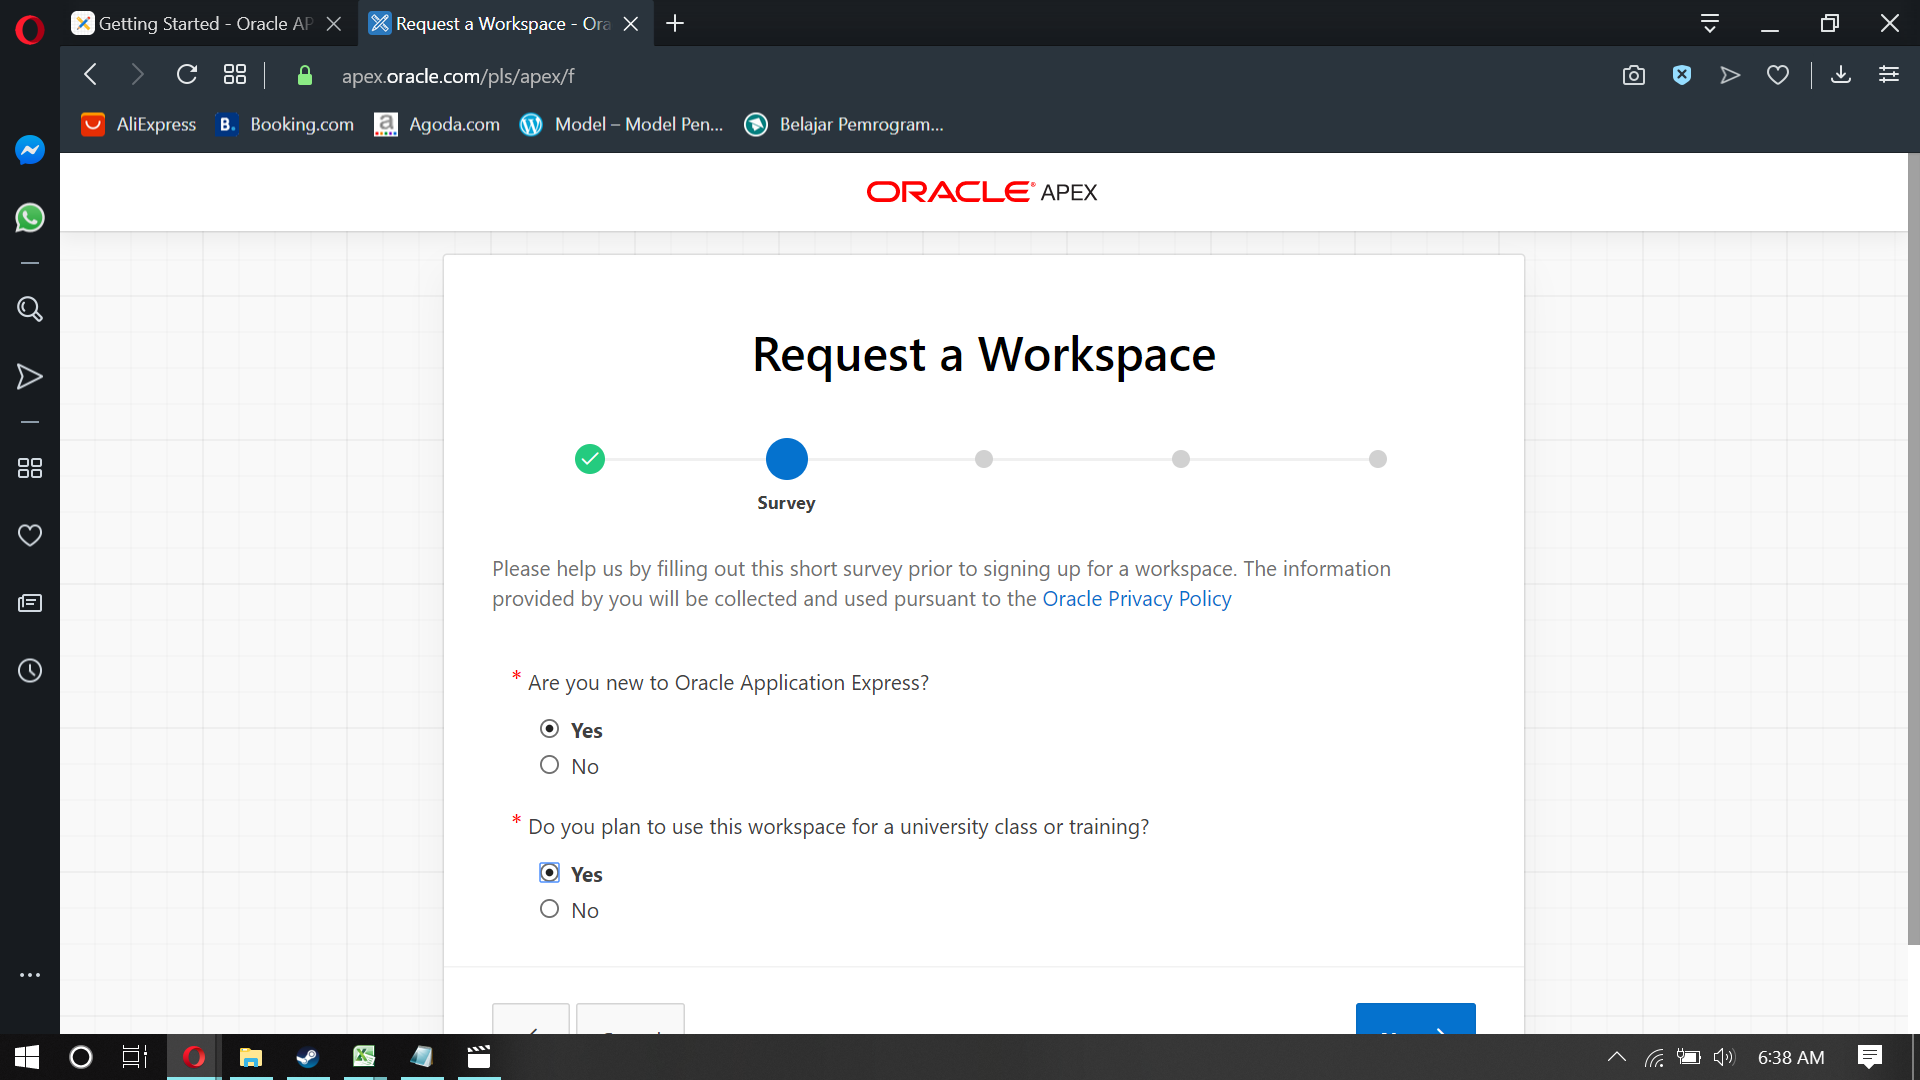
\includegraphics[width=12cm]{gambar/Screenshot (109).png} 
	\item isi form sesuai kebutuhan, lalu klik next\\	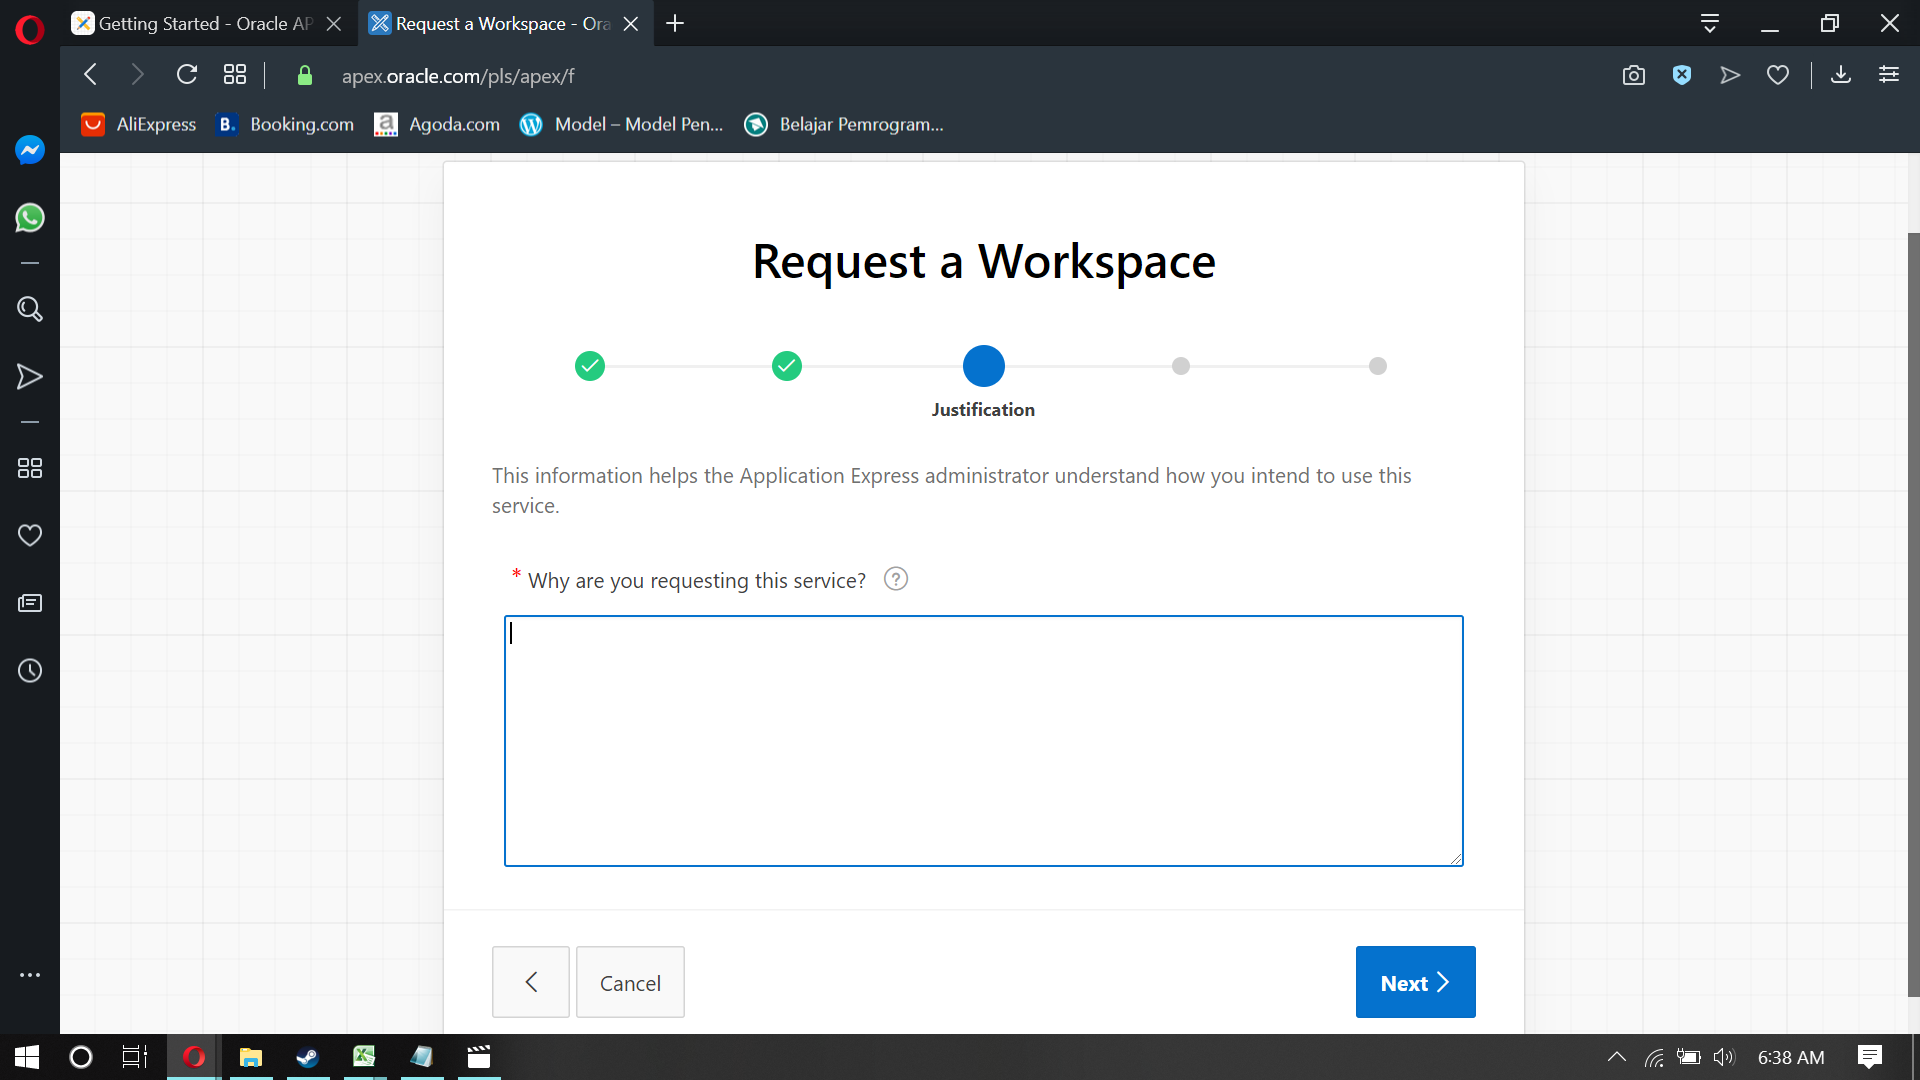
\includegraphics[width=12cm]{gambar/Screenshot (110).png} 
	\item cetang accept, lalu klik next\\	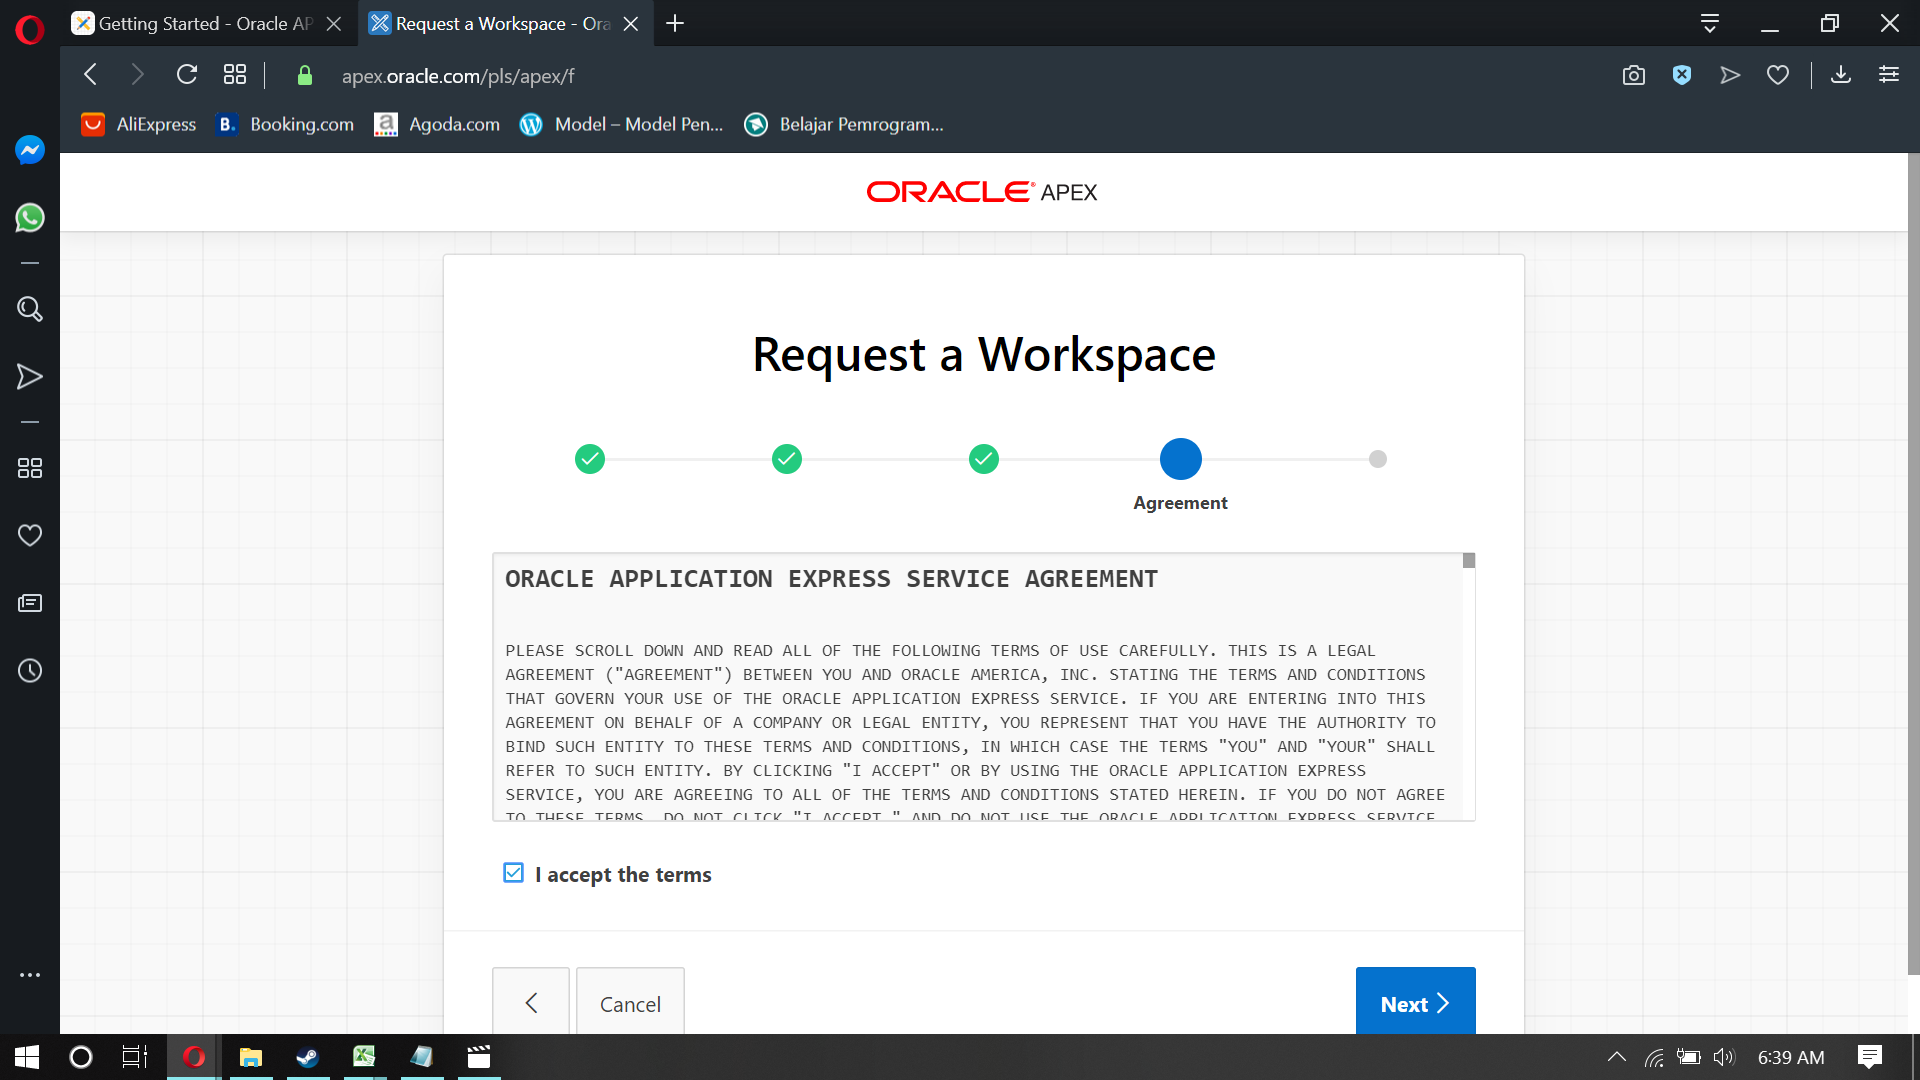
\includegraphics[width=12cm]{gambar/Screenshot (111).png} 
	\item klik submit request\\	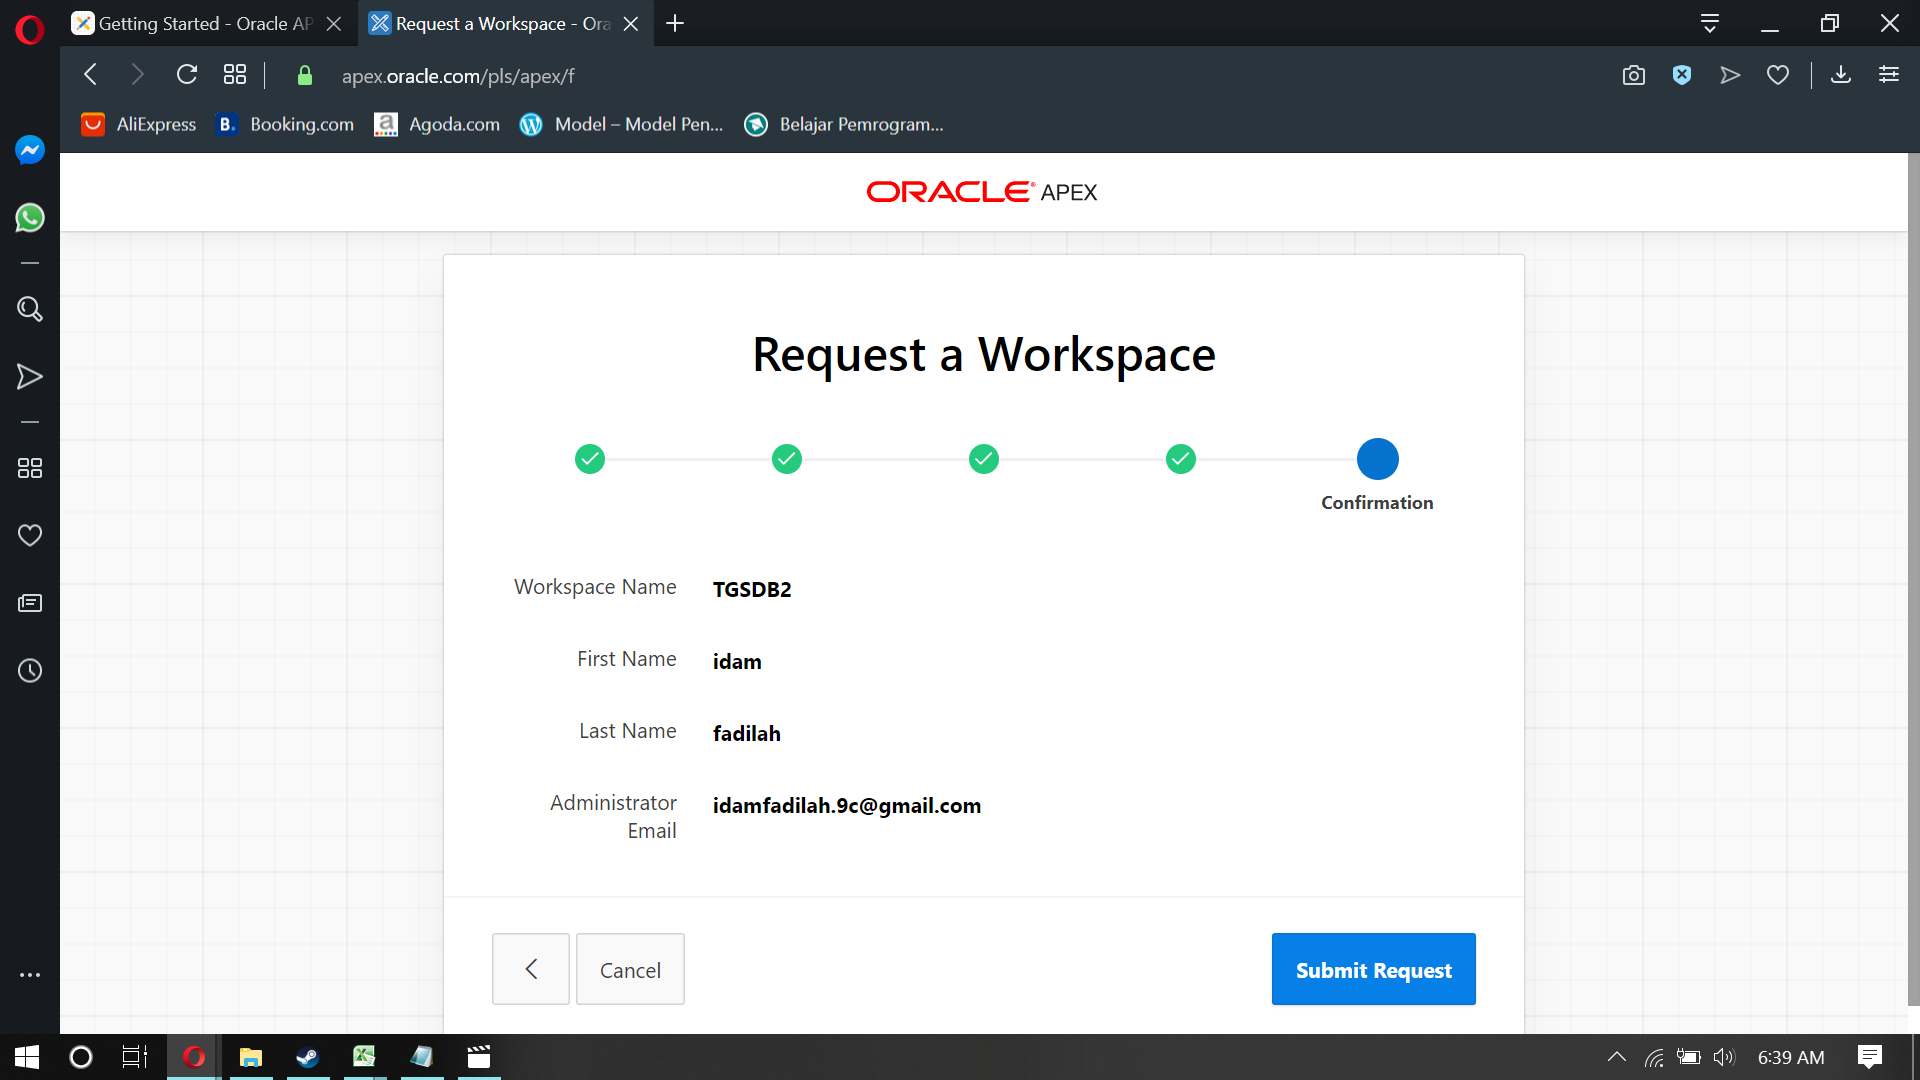
\includegraphics[width=12cm]{gambar/Screenshot (112).png} \\	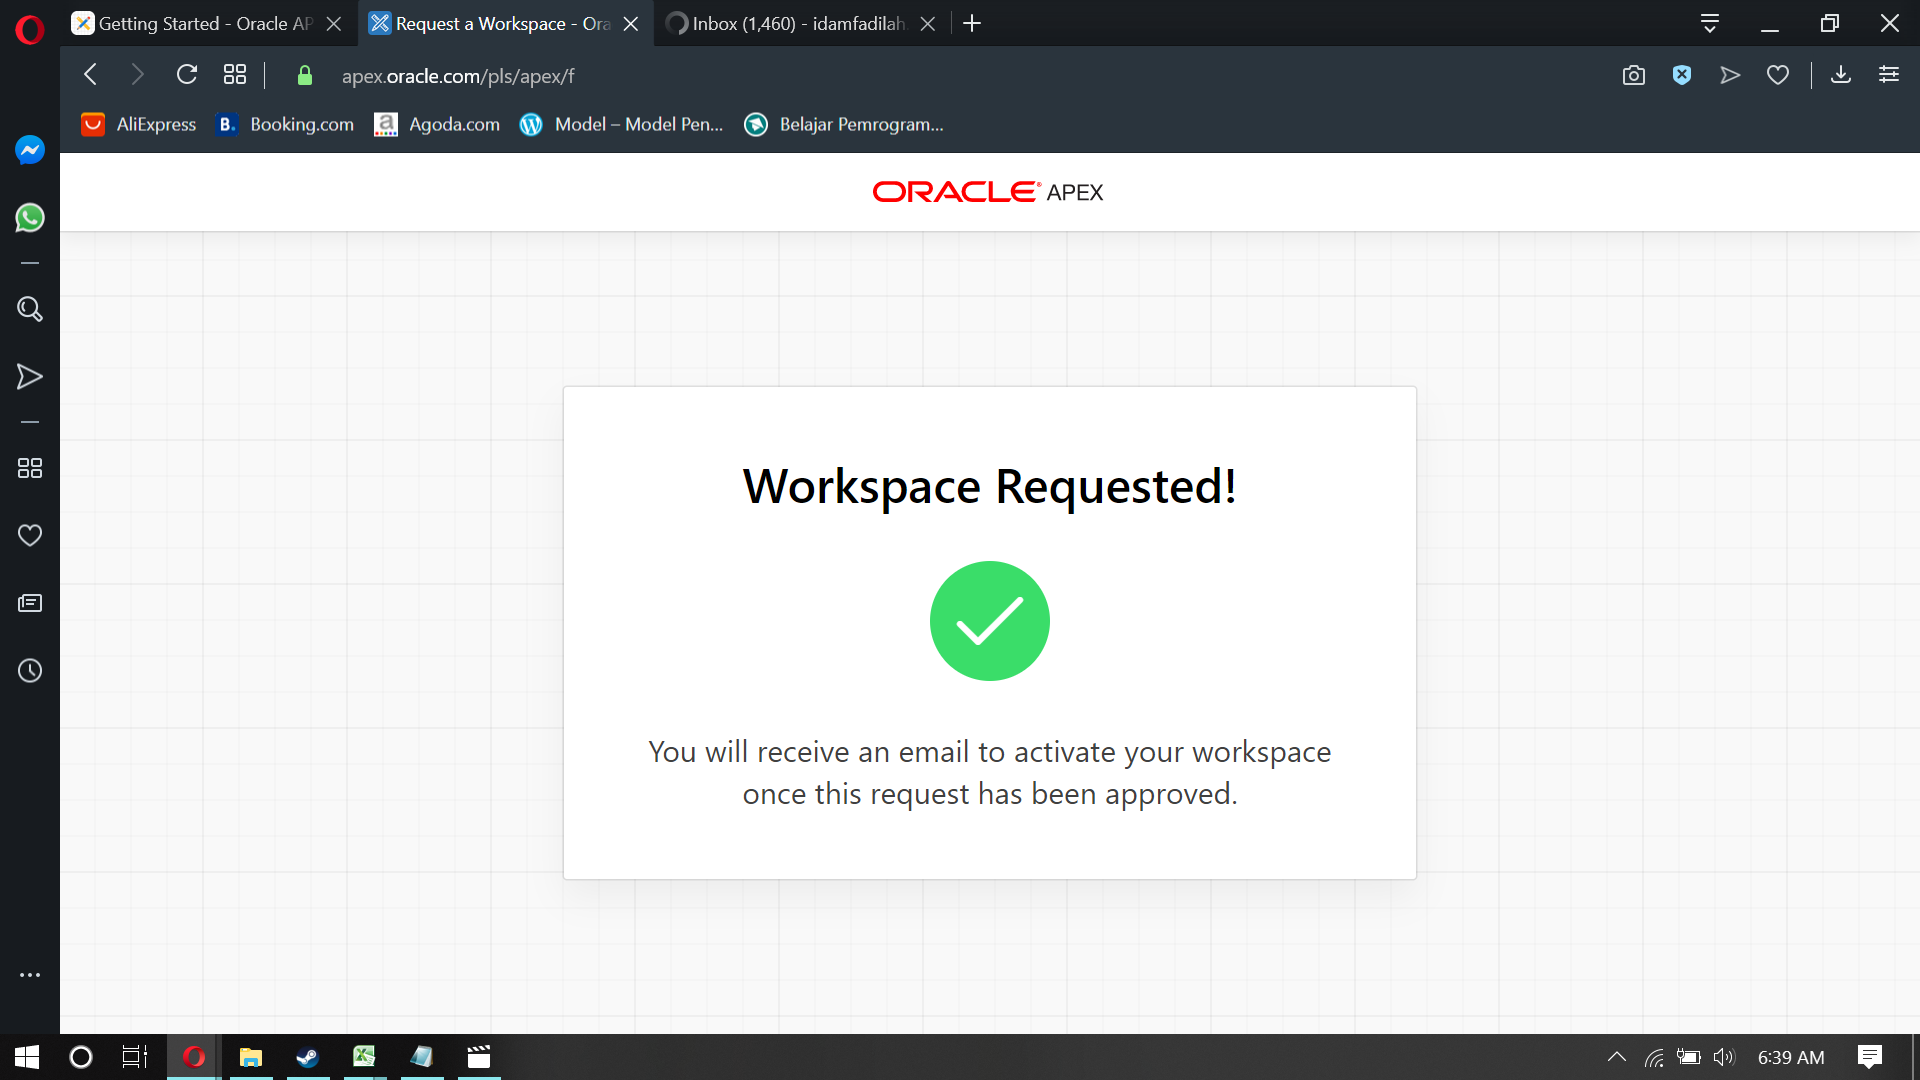
\includegraphics[width=12cm]{gambar/Screenshot (113).png} 
	\item buka email dari oracle lalu klik create workspace\\ 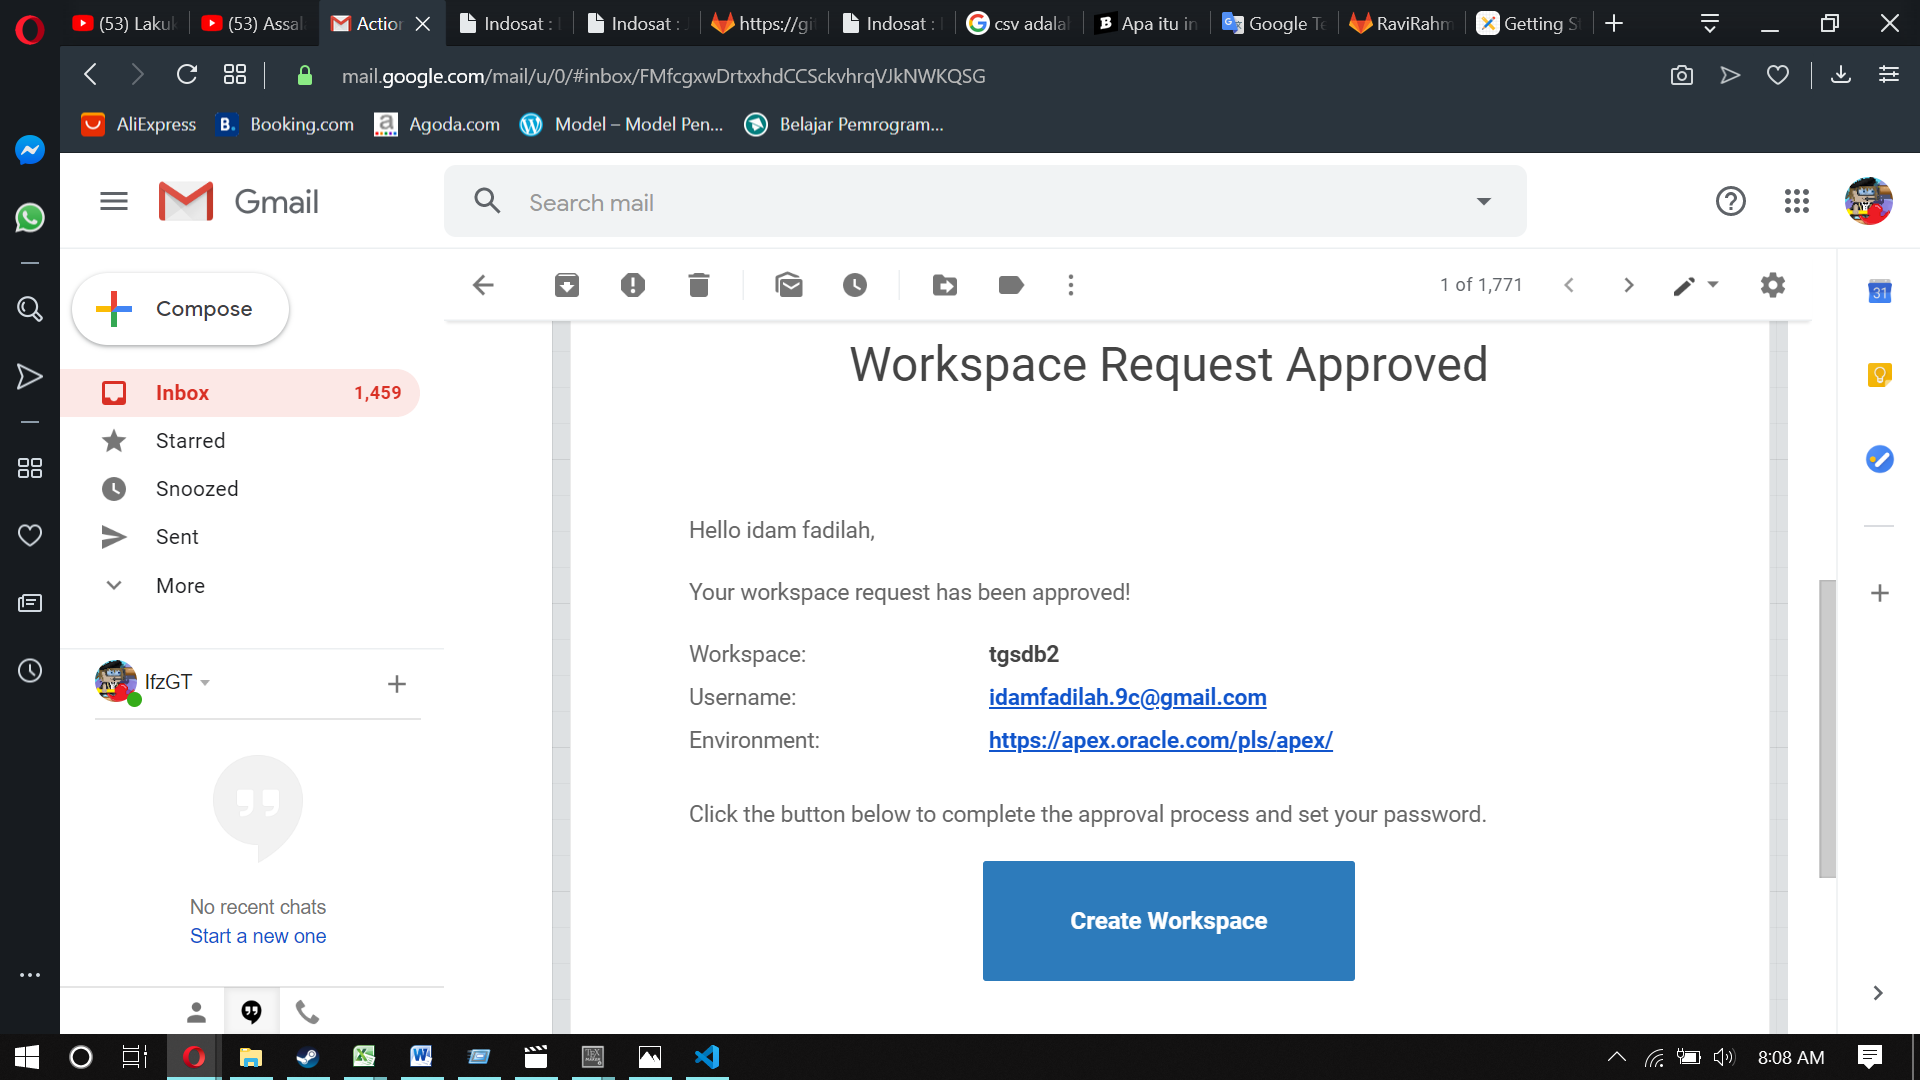
\includegraphics[width=12cm]{gambar/Screenshot (119).png} 
	\item lalu login ke Oracle APEX, dengan data yang sudah didaftarkan\\
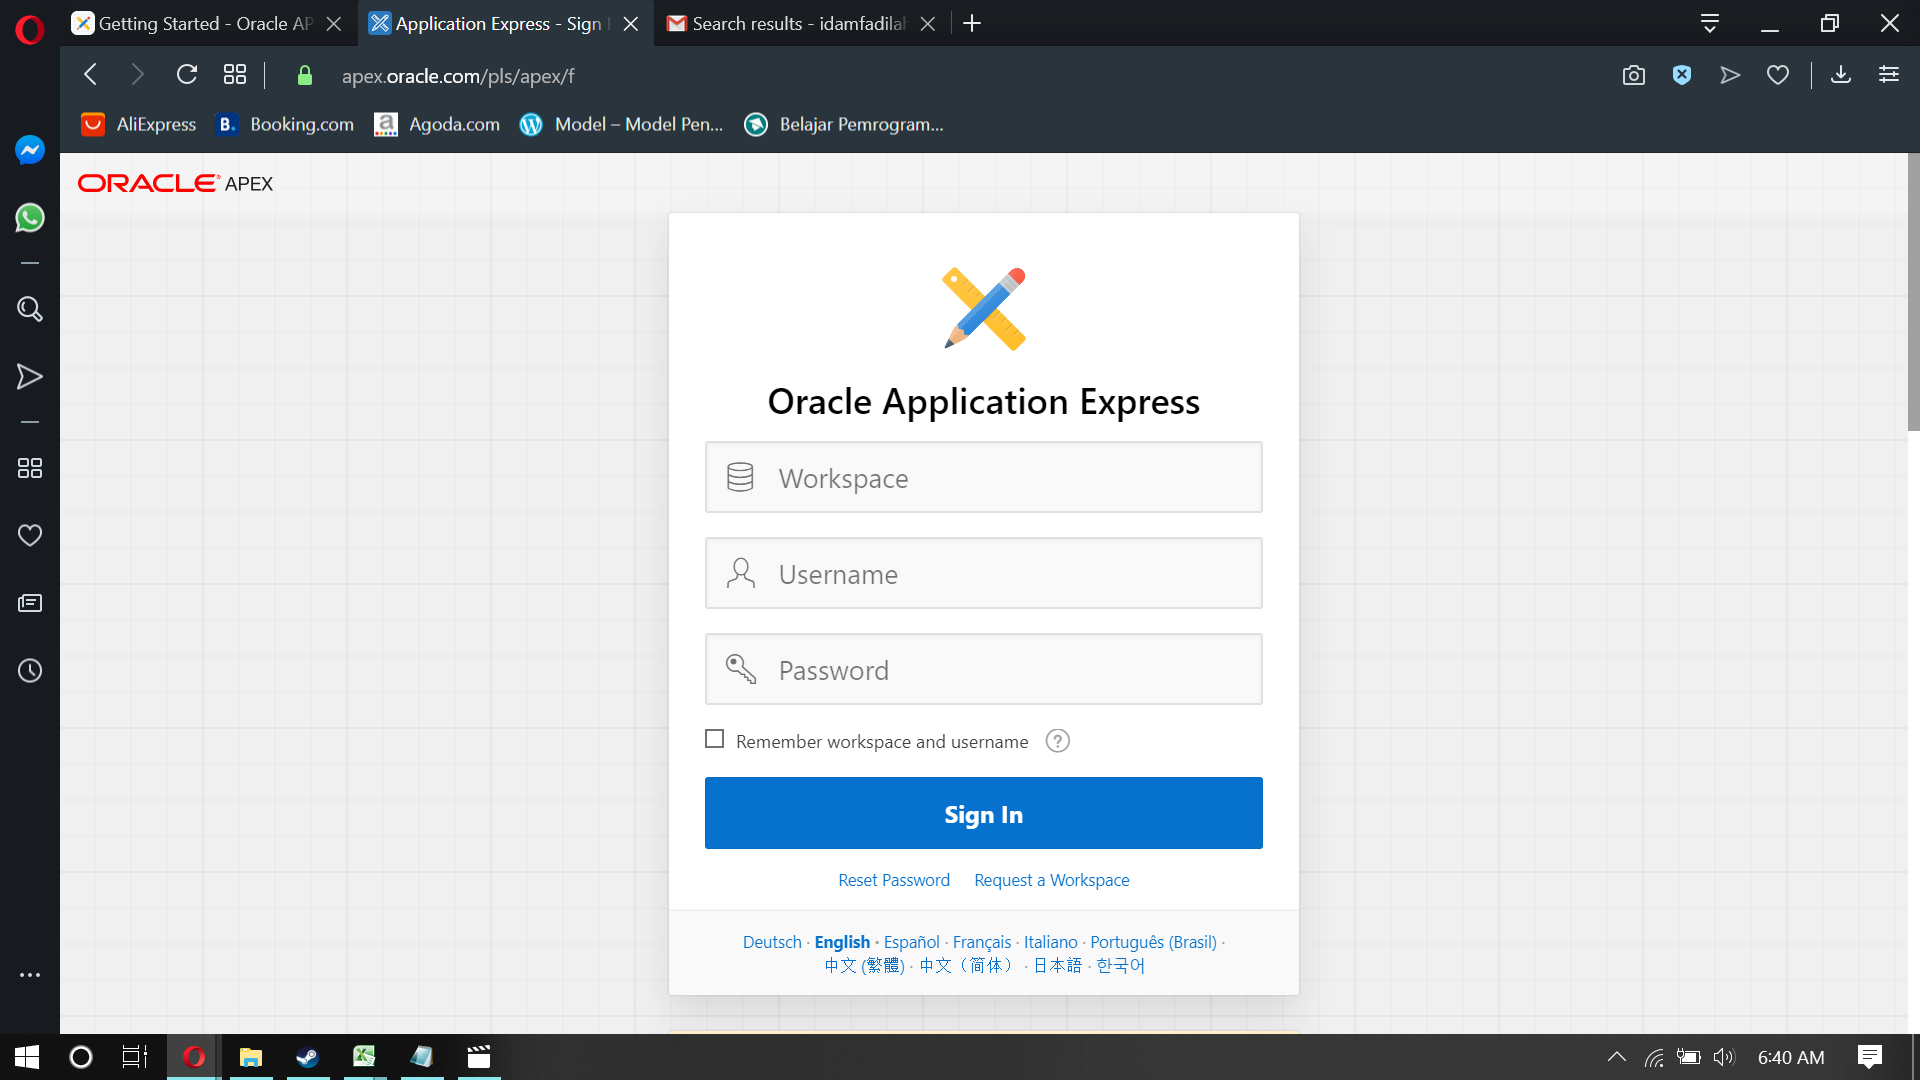
\includegraphics[width=12cm]{gambar/Screenshot (114).png} 
	\item tampilan sesudah login, selesai\\
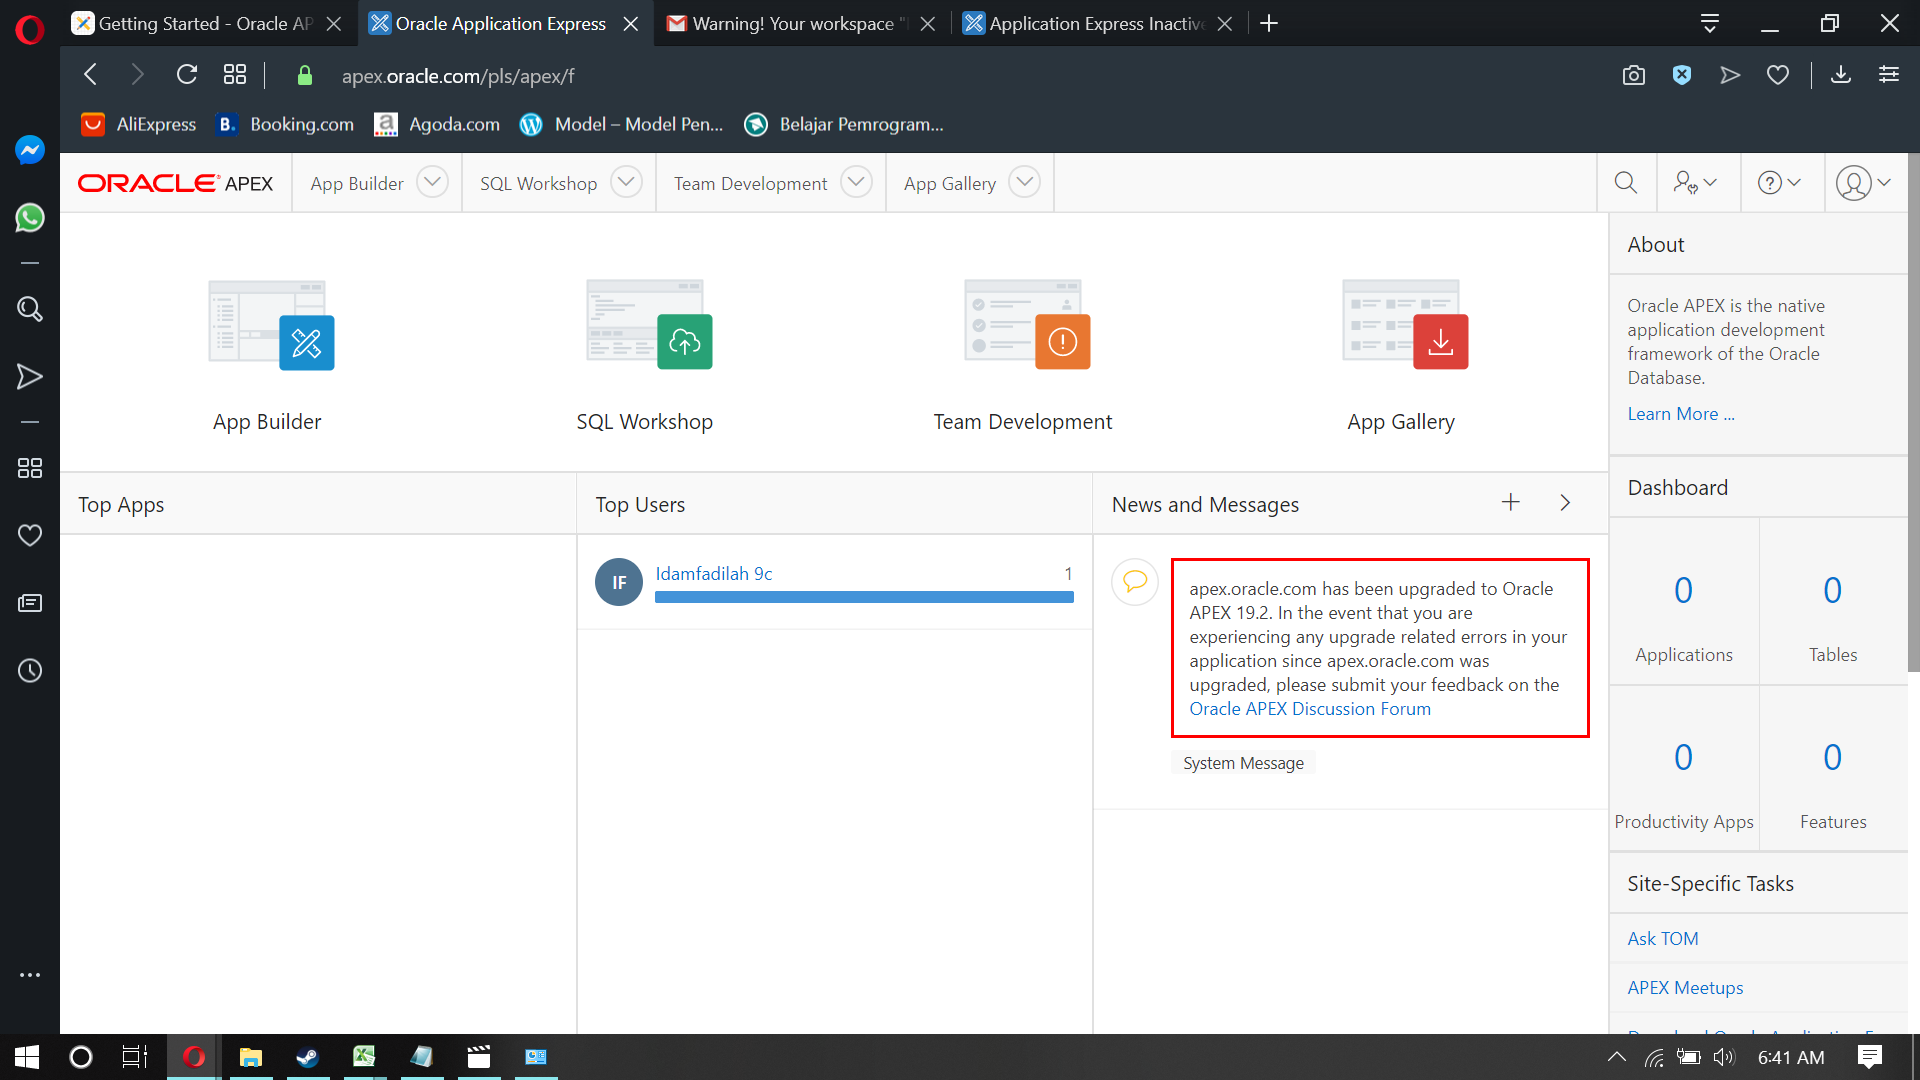
\includegraphics[width=12cm]{gambar/Screenshot (115).png} 
\end{itemize}


\end{document}
